%\RequirePackage{luatex85}
\documentclass[11pt]{scrreprt}

%\usepackage{fontspec}
\usepackage{amsmath,amssymb}
\usepackage{mathpazo}
\usepackage{XCharter}
\usepackage{cabin}
\usepackage[utf8]{inputenc}
\usepackage[T1]{fontenc}
\usepackage[dvipsnames]{xcolor}
\usepackage{csquotes}
\usepackage{marginnote}
\usepackage{tikz}
\usepackage{pgfplots}
\usepackage{pgfplotstable}
\pgfplotsset{compat=newest}
\usepackage{graphicx}

\usepackage{geometry}
\usepackage[ngerman]{babel}
%\defaultfontfeatures{Ligatures=TeX}
% Set sans serif font to Calibri
%\setsansfont{Calibri}
% Set serifed font to Cambria
%\setmainfont{Cambria}
% Define light and dark Microsoft blue colours
\definecolor{MSBlue}{rgb}{.204,.353,.541}
\definecolor{MSLightBlue}{rgb}{.31,.506,.741}
\addtokomafont{chapter}{\color{MSBlue}}
\addtokomafont{section}{\color{MSBlue}}
\addtokomafont{subsection}{\color{MSLightBlue}}

\addtokomafont{caption}{\sffamily}
\addtokomafont{captionlabel}{\usekomafont{caption}\bfseries\color{MSBlue}}

\usepackage[backend=biber,style=alphabetic,hyperref=true,backref=true,block=none,url=false,isbn=false,doi=false,maxcitenames=3,maxbibnames=100]{biblatex}
\addbibresource{references.bib}

\title{Die bunte Welt der Farbstoffe}
\author{Lukas Braun}
\publishers{
\includegraphics[width=5cm]{logo.jpg} \\ Descartes Gymnasium Neuburg a. d. Donau}
\subject{Chemie}
\subtitle{W-Seminar -- Chemisch Kochen}
\date{07. Oktober 2016}

\usepackage[automark]{scrlayer-scrpage}
\usepackage[onehalfspacing]{setspace}
\emergencystretch=.5em
\renewcommand*{\dictumauthorformat}[1]{(#1)\vspace*{1em}}


\usepackage{siunitx}

\usepackage{abstract}
\setlength{\absleftindent}{3cm}
\setlength{\absrightindent}{3cm}
\setlength{\absparindent}{0cm}

\usepackage{hyperref}
 
\begin{document}
\renewcommand{\abstractname}{Abstract}
\maketitle
\clearpage
\newgeometry{
	a4paper,
	left=30mm,
	right=20mm,
	top=25mm,
	bottom=25mm
}

\begin{abstract}
	\noindent

\end{abstract}

\clearpage
\tableofcontents
\clearpage
\listoffigures
\clearpage
\chapter{Geschichte der Lebensmittelfarben}
Unser ganzes Leben werden wir von Sinneswahrnehmungen unserer Augen überflutet. In der Natur hat jede einzelne Farbe, die wir Menschen wahrnehmen eine Bedeutung. Leuchtend starke Farben dienen meist als Signal, mit den natürlichsten Zielen der Natur- und Pflanzenwelt: Einerseits sollen Tiere vor einer Gefahr gewarnt werden. Dies geschieht zumeist in einer Farbkombination aus Gelb und Schwarz. Als Beispiel hierfür kann die Echte Wespe herangezogen werden, die mit ihren schwarz-gelbem Körper möglichen Fressfeinden eine Gefahr signalisiert. Als zweites wichtiges Ziel von Signalfarben gilt die Vermehrung, so ist das farbenfrohe Gefieder von Vögeln während der Balz oder die Blüten von Rosen ein Lockmittel für bestäubende Tiere oder einen möglichen Sexualpartner. 

\begin{figure}[ht!]
	\centering
	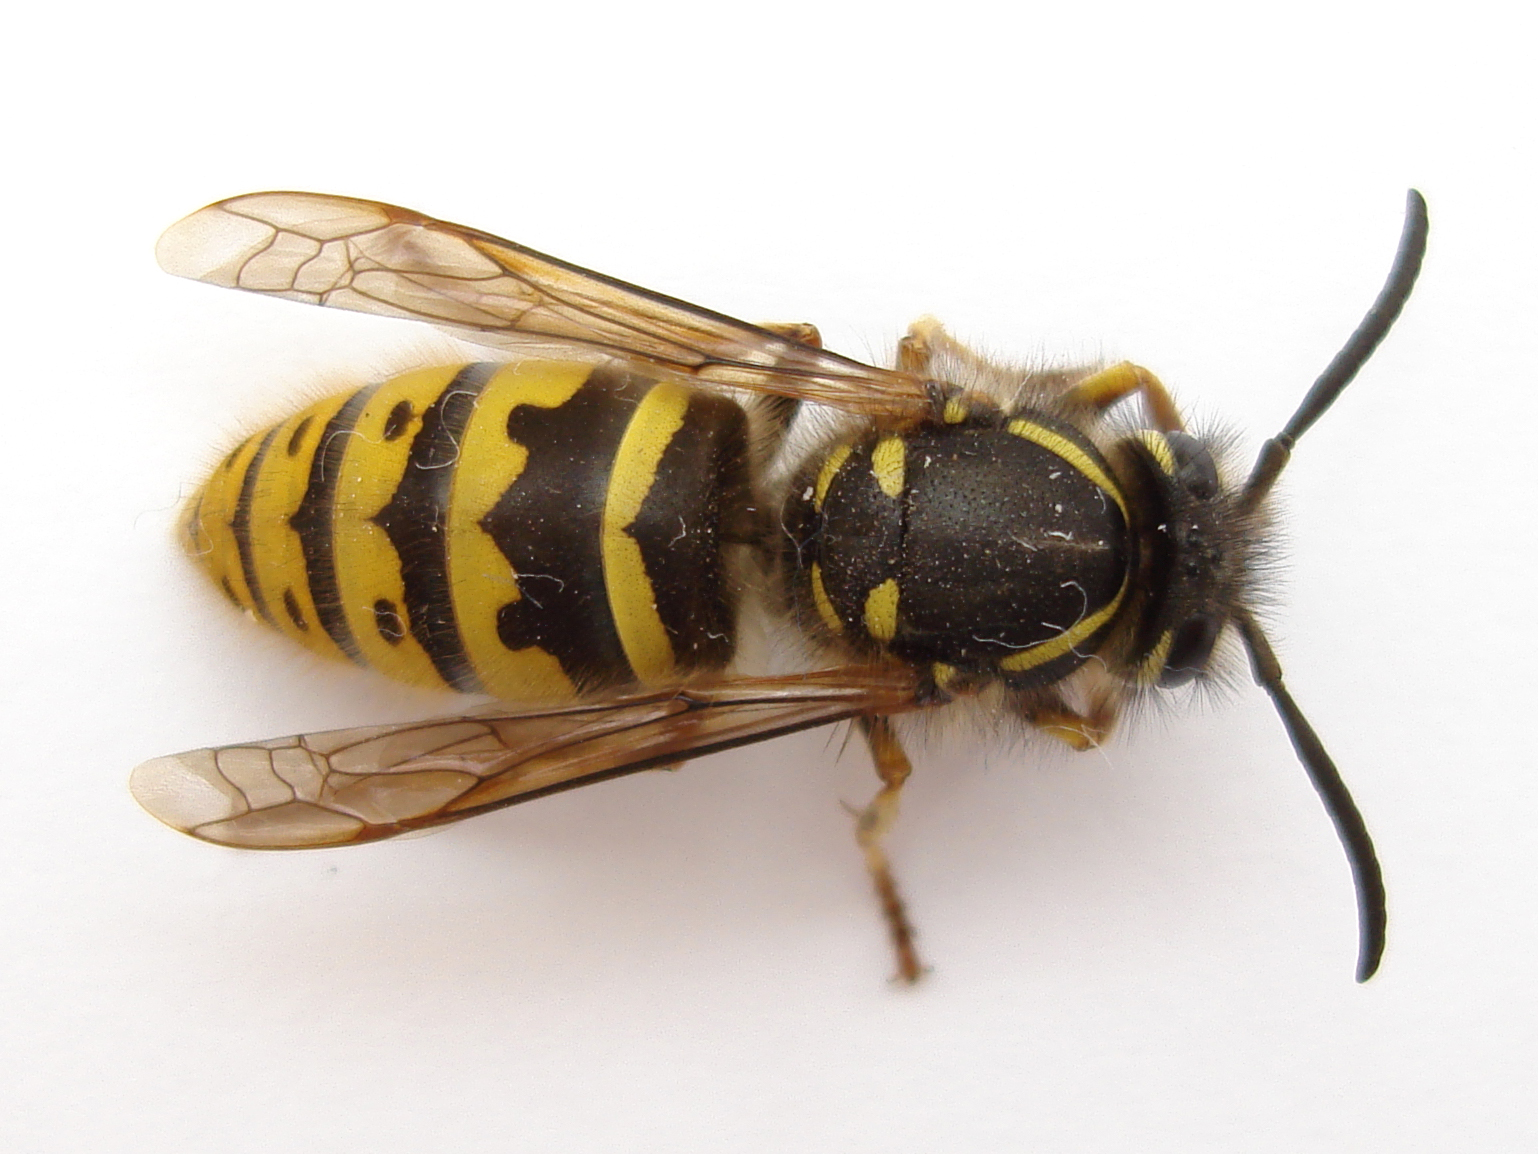
\includegraphics[width=0.4\textwidth]{wespe.jpg}
	\caption[Eine Wespe als Beispiel für Signalfarben, das Bild wurde vom Nutzer \textit{Trounce} über die Wikimedia Commons zur Verfügung gestellt.]{Eine Wespe als Beispiel für Signalfarben}
	\label{img:wasp}
\end{figure}

Auch Menschen reagieren sehr stark auf die Farben der Umwelt, so verbinden wir ein bestimmtes Lebensmittel meist mit genau einer Farbe. Denn wer assoziiert Himbeeren mit einer anderen Farbe als einem leuchtenden Rot? Dieses Verhalten hat sich im Menschen über Jahrtausende durch Traditionen und der Umwelt eingeprägt. Auch heute noch wird bei einem Einkauf zunächst die Farbe der Lebensmittel überprüft. Sie gibt die Reife und somit eine Erwartung an Geschmack, Geruch und Inhaltsstoffe an. Deshalb werden zur Entwicklung von modernen Lebensmitteln bereits Farbpsychologen benötigt und in einem Supermarkt die Früchte mit speziellem Licht bestrahlt, um sie für den Kunden ansprechender wirken zu lassen\cite[S. 88ff]{Hamatschek.2016}..

Bereits um 1500 vor Christus färbten ägyptische Händler ihre Süßigkeiten, indem sie natürliche Pflanzenextrakte und Wein hinzufügten Von dort aus verbreitete sich diese Methode über das römische Reich. Diese Vorgehensweise ging im Mittelalter jedoch größtenteils verloren, da das Aussehen der Lebensmittel für die verarmte Bevölkerung vergleichsweise unbedeutend gewesen ist\cite{HarryMeggos.1995}. Dies änderte sich erst bei Bildung von größeren Städten in der frühen Moderne. Der internationale Handel nahm zu, und es werden vermehrt exotische Gewürze und Färbemittel nach Europa importiert. So wurde bereits 1531 ein Gesetz in Augsburg erlassen, dass Fälscher von Safran mit dem Tode bestraft und allgemeine Regeln für Gewürze und Farbstoffe bestimmt.

Durch die industrielle Revolution im 19. Jahrhundert stieg die Nachfrage nach günstigen Lebensmitteln stark an. Zu dieser Zeit war die Analytische Chemie noch in ihren Kinderschuhen, sodass noch keine Lebensmittelkontrollen existierten, die den heutigen Standards ansatzweise entsprechen.  Demzufolge kann es heutzutage keinen mehr wundern, dass die Streckung von Lebensmitteln florierte. Schwermetalle und andere anorganische Stoffe stellten einen kostengünstigen Ersatz dar, um die ursprüngliche Farbe von verdünnter Milch und anderen Lebensmitteln wiederherzustellen. Mit Bleioxid können beispielsweise Käse und Süßwaren gefärbt werden\cite{Natcol.2016,Downham.2000}.Erst im Jahre 1959 wurde in Deutschland die Farbstoff-Verordnung erlassen. Seitdem gelten in Deutschland strengere Maßstäbe bezüglich der Unbedenklichkeit von Lebensmittelzusatzstoffen. Nur noch einige Chemikalien, die auf einer Positivliste enthalten sind, dürfen noch verwendet werden. Eine weitere Verschärfung dieser Regelung erfolgte 1977 mit der Zusatzstoff-Zulassungsverordnung. Ab diesem Zeitpunkt müssen alle enthaltenen Zusatzstoffe klar deklariert sein\cite[S.48-49]{Heinze.1986}.


%Lebensmitteltechnologie Jochen Hamatschek 2016 S.88 ff
%Food colours: an international perspective von Meggos h 59 ff
%http://natcol.org/library/introduction-food-colours-legislation/ aufgerufen am 03.10.2016
%http://www.blacksci.co.uk/products/journals/freepdf/tmp1.pdf aufgerufen am 08.09.2016
%(doi:doi:10.1046/j.1365-2621.2000.00373.x. )
%http://jama.jamanetwork.com/article.aspx?articleid=465550 Artikel: Human food laws aus "The Journal of the American Medical Association. Chicago: American Medical Association." ausgabe 1898 Nr 8 von Robert W. Hastings
%http://www.fda.gov/AboutFDA/WhatWeDo/History/FOrgsHistory/CFSAN/ucm083863.htm   von U.S. Food and Drug Administration Titel: "A Century of Ensuring Safe Foods and Cosmetics"
%
\chapter{Definition von Farben}
\section{Eigenschaften }
\dictum[Sprichwort]{%
	Nachts sind alle Katzen grau.
}
Um Farben sehen zu können, wird Licht benötigt, denn wie das Sprichwort sagt, sind nachts alle Katzen grau.  Doch was ist Licht? Um diese Frage genauer zu erklären, ist zunächst ein kleiner Exkurs in die Physik notwendig. Das \enquote{weiße} Licht der Sonne ist im Grunde eine Überlagerung von elektromagnetischer Schwingungen mit unterschiedlichen Wellenlängen $\lambda$. Hierzu betrachten wir zunächst ein Prisma aus Glas, in welchem weißes Licht aufgebrochen wird und ein Farbspektrum, vergleichbar mit einem Regenbogen, entsteht. Abhängig von der Wellenlänge wird das Licht im Prisma unterschiedlich stark gebrochen und somit das typische Farbspektrum sichtbar.  Das für den Menschen sichtbare Licht hat eine Wellenlänge zwischen \SI{400}{\nano\meter}  bei violetten Licht und \SI{800}{\nano\meter} bei rotem Licht. Die Wellenlänge des Lichtes bestimmt die Farbe und den Energiegehalt.

\begin{equation}
	E = h \frac{c}{\lambda}
\end{equation}

 So liegt die Energie des sichtbaren Lichts zwischen  \SI{1,6}{\electronvolt} bei rotem und  \SI{2,4}{\electronvolt} bei blauem Licht. Dieser Teilbereich der Physik wurde bereits in der Antike unter anderem von Ptolemäus und Archimedes erforscht.

Licht entsteht, indem zunächst Elektronen innerhalb der Atome durch die Zufuhr von Energie angeregt werden und dadurch auf eine bestimmte, höhere Energiestufe\footnote{ Entspricht einer höheren Geschwindigkeit und einer größeren Entfernung zum Atomkern} angehoben werden. Da dieser Zustand relativ energiereich und  instabil ist, fällt das Elektron auf sein ursprüngliches Energieniveau zurück. Die daraus resultierende Energiedifferenz kann, abhängig vom Molekülbau, als Wärmestrahlung oder als Lichtstrahlung abgegeben werden. Die Größe der Energiedifferenz entscheidet zudem über die Farbe des ausgesandten Lichts: Bei einer größeren Energie, wird eine kurzwelligere Strahlung emittiert.

Tritt nun Licht auf einen Körper, so können verschiedene, stoffspezifische Ereignisse auftreten: Durch diese elektromagnetische Strahlung werden Elektronen auf ihr nächsthöheres Energieniveau gehoben und beim Zurückfallen Licht ausgesandt. Dieses Phänomen wird Remission genannt. 

Eine andere Möglichkeit ist, dass nicht die genau benötigte Energiemenge an den Körper geraten und die Elektronen kein höheres Energieniveau erreichen. Die Energie wird nun nur in Form von Wärme emittiert. Jeder Stoff kann jedoch nur Licht bestimmter Wellenlängen absorbieren. Die restlichen Wellenlängen werden reflektiert, und durch additive Mischung dieser Wellenlängen resultiert die für den Menschen erscheinende Eigenfarbe des Stoffes\cite[S.9-15]{Jenette.1983}.

\section{Färbung organischer Stoffe}
\section{Färbung anorganischer Stoffe}

%\begin{figure}[ht!]
%	\centering
%	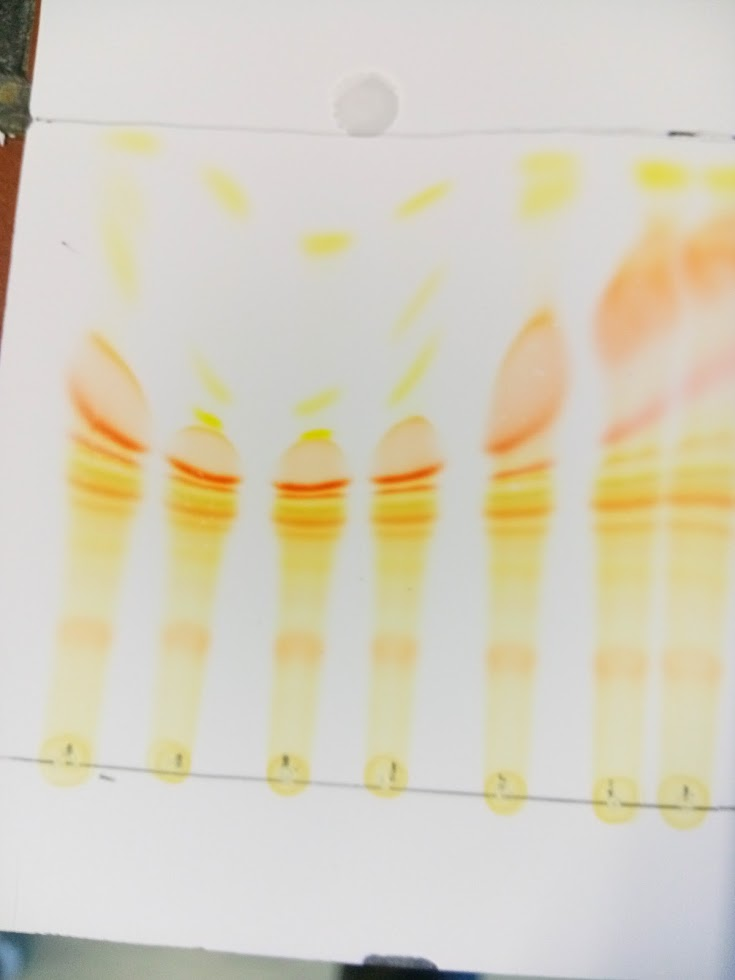
\includegraphics[width=\textwidth]{paprika.jpg}
%	\caption{Entstehung der Farbigkeit eines stoffes}
%	\label{img:Reflektion und Addition von Licht}
%\end{figure}n
\chapter{E-Nummern}
Wenn man sich längere Zeit mit Farbstoffen in Lebensmitteln beschäftigt, fällt der Blick auch auf die sogenannten \enquote{E-Nummern}. Hierbei handelt es sich um eine Liste von über 300 zugelassenen Zusatzstoffen in Lebensmitteln. Diese Liste wird von der European Food Safety Autority\footnote{kurz EFSA} unter der Berücksichtigung von \enquote{allen verfügbaren, einschlägigen wissenschaftlichen Studien}erstellt, mit dem Ziel, einen freien Warenverkehr innerhalb der Europäischen Union zu ermöglichen \cite{EFSAisanagencyoftheEuropeanUnion.2016}.

Doch warum benötigt es eine eigene Benennung von Chemikalien, speziell für Europa?
Dies lässt sich recht einfach anhand eines Beispiel erklären: Der Lebensmittelfarbstoff E120 besitzt allein in Deutschland fünf unterschiedliche Bezeichnungen: Cochenille, Karmin, Karminsäure, Echtes Karmin und Karminrot sind Synonyme  für den ausgekochten Farbstoff von weiblichen Schildläusen. Da in jedem einzelnen EU-Land eigene Begriffe hierfür vorhanden sind, können die Verbraucher schwer den Inhaltsstoff bestimmen.
Des Weiteren galten in den EU-Mitgliedsländer vor 1993, dem Jahr der Einführung von E-Nummern, jeweils eine eigene Liste von erlaubten Zusatzstoffen in Lebensmitteln. Dadurch war der Warenverkehr erschwert, da ein Hersteller die Inhaltsstoffe sowohl die Gesetzgebung des Produktionslandes als auch des Verkaufslandes berücksichtigen muss. Seit der Einführung der europaweiten Regelung sind zudem größtenteils nur farbverstärkende, anstatt von farbverändernde Stoffe erlaubt. Die Täuschung über die eigentlichen Inhaltsstoffe ist dadurch erschwert.

 Durch die stetigen Kontrollen soll vor allem die Verträglichkeit der Lebensmittel gewährleistet werden. Dies erfolgt zum Beispiel durch das Prüfen von allen vorhandenen Studien bezüglich der Nebenwirkungen und Toxizität von Stoffen. Hierbei sind in den letzten Jahren vor allem sogenannte Azofarbstoffe in den Verdacht geraten das Aufmerksamkeits-Defizits-Syndrom und Allergien auszulösen.  Sie müssen seit dem 20.07.2010 den Warnhinweis \enquote{Kann Aktivität und Aufmerksamkeit von Kindern beeinträchtigen} tragen und werden weiterhin kritisch betrachtet. Einige Abkömmlinge der Azofarbstoffe wurden überdies als krebserregend eingestuft, und sind  deshalb sowohl in Lebensmitteln  als auch in Kleidung verboten. Da sie allerdings überdurchschnittlich gute Färbeeigenschaften besitzen, wie starke leuchtende Farbigkeit, Lichtunempfindlichkeit, Säurestabilität Wasserlöslichkeit sowie Hitzebeständigkeit, werden sie auch heute vielfältig verwendet\cite[S.50]{Heinze.1986}. Deshalb ist stets ein geschulter Blick auf die Inhaltsstoffe empfehlenswert, wobei natürlich auch hier der Grundsatz gilt, dass \enquote{die Dosis das Gift macht}.

 \cite[S. 12]{Schobert.2007}. 
 
 
\chapter{Farbstoffextraktion}
Jedoch ist nicht jedes Lebensmittel nicht ausreichend oder gar nicht mit den enthaltenen Farbstoffen deklariert. Für diesen Fall bietet die Chemie jedoch verschiedene Möglichkeiten zur Überprüfung der Inhaltsstoffe. Hier wäre in der freien Wirtschaft vor allem die Hochleistungsflüssigkeitschromatographie zu nennen. Für kleinere Untersuchungen mit wenigen farbigen Inhaltsstoffen ist eine Dünnschichtchromatografie\footnote{kurz DC} ausreichend. Für diese, seit 1903 von Tswett entwickelte und von da an stets verbesserte Methode benötigt man nur wenige Milliliter der Probesubstanz. Sie ist zudem sehr kostengünstig realisierbar und kann auf nahezu jeden Stoff angewendet werden. Der Aufwand an benötigten Gerätschaften ist zudem vernachlässigbar. Problematisch ist jedoch, wenn die Probe zu viele verschiedene Farbstoffe enthält, da ab etwa zehn verschiedenen Farbstoffen kein klares Ergebnis erkennbar ist. Zudem können keine quantitativen Untersuchungen stattfinden. Dennoch handelt es sich um eine sinnvolle Farbstofftrennmethode,die aus diesem Grund  an Schulen und Universitäten gelehrt wird. Ziel der Dünnschichtchromatografie ist meist $\mu$ der stoffspezifische Rf- Wert (\enquote{Ratio of front}).  Er gibt das Verhältnis der Laufmittelfront und der Fließhöhe des Stoffes an. Hierzu jedoch später mehr\cite[S.117-123]{Wittke,1984}.

 \section{ Anleitung für eine  Dünnschichtchromatografie} 
 
 Zunächst wird die Substanz auf die feste Phase mithilfe einer Kapillare aufgetragen. Die stationäre Phase  besitzt eine dünne Trennschicht,, zum Beispiel aus Kieselgel,  die auf einer Trägerplatte wie Kunststoff oder Aluminium aufgetragen ist. Man sollte zum einem einen Abstand von circa \SI{1}{\centi\meter} zu allen Rändern und zwischen den einzelnen Probesubstanzen einhalten. Diese Stelle auf der Dünnschichtplatte wird auch Startlinie genannt. Als Hilfe wird oft eine Markierung mit einem Bleistift oder Ähnlichen empfohlen, der unter Umständen das Ergebnis verfälschen kann.  Um diesen Schritt zu vereinfachen sind Schablonen im Fachmarkt erhältlich, bei denen allerdings mit stark flüchtigen Lösungsmitteln gearbeitet werden sollte. Die angefertigte DC-Platte sollte man nun trocknen lassen, sodass nur noch wenig Lösungsmittel enthalten ist. Darauf folgt die Herstellung des Fließmittels. Falls es sich um giftige Chemikalien handelt, sollten unbedingt eine Schutzbrille sowie Latexhandschuhe getragen werden und der gesamte Versuch ab sofort unter einer Abzugshaube fortgeführt werden. Das Fließmittel dient als Transportmedium für die Substanz.
 
 Nun füllt man die Dünnschichtkammer 0,5 bis \SI{1}{\centi\meter} mit diesem Laufmittel auf. Die Höhe variiert durch die verwendete Starthöhe auf der Dünnschichtplatte, da das Fließmittel nicht sofort in Kontakt mit der zu untersuchenden Substanz treten soll. Um eine hohe Luftsättigung innerhalb der Dünnschichtkammer zu erreichen ist es empfehlenswert die Kammer leicht zu schütteln,oder die Kammer mit Filterpapier auszulegen. Gleich darauf gibt man die Dünnschichtplatte mit der Starthöhe unten in die Dünnschichtkammer und schließt diese daraufhin mit einem gut gefetteten Deckel. Jetzt wartet man bis entweder die mit den Vergleichs"=RF"=Werten angegebene Zeit verstrichen ist, oder, falls man eine eigene \enquote{Vergleichsdünnschichtchromatografie} durchführt, bis eine sehr gute Trennung der Substanzen erkennbar ist. Auf jeden Fall darf die Laufmittelfront, die maximale Höhe des Laufmittels, nicht das obere Ende der DC-Platte erreichen, da somit kein richtiger RF-Wert mehr errechnet werden kann. Nach Erreichen der gewünschten Trennung wird die Platte aus der Kammer entfernt und sofort die Laufmittelfront und die aufgetrennten Farbstoffe gekennzeichnet, da sich das diese Substanzen verflüchtigen können und so das Ergebnis verfälscht wird. 
 Die feste Phase sollte man jetzt trocknen lassen. Abhängig von der verwendeten Probesubstanz kann eine Untersuchung unter ultraviolettem Licht durchgeführt werden, um weitere Chemikalien sichtbar zu machen. Auch kann die gesamte Platte mit einer Farbe eingefärbt werden, wie zum Beispiel einem Indikator, der sich bei farblosen Säuren oder Basen verfärbt sodass diese  erkennbar sind. Daraufhin hat man mit der Berechnung der RF-Werte die Dünnschichtchromatografie vollständig abgeschlossen\cite[S.117-118]{Wittke,1984}.

 \section{Die chemischen und phsyikalischen Vorgänge einer Dünnschichtchromatografie}
 Für die Durchführung einer Dünnschichtchromatografie benötigt man eine stationäre, beziehungsweise feste Phase, hier verwendet man bevorzugt eine Kieselgelplatte. Sie dient als Übergangsträger für die zu untersuchende Substanz.
Bei Kieselgel handelt es sich um ein Siliziumsalz, das eine sehr große Oberfläche aufweist, um eine große Menge der Substanz temporär aufzunehmen. Zudem können sowohl leicht polare als auch unpolare Moleküle als Untersuchungssubstanz verwendet werden. Als Alternative wäre vor allem eine Aluminiumoxidplatte zu nennen, die jedoch als Katalysator für manche Reaktionen dienen kann und somit den Molekülbau verändern könnte. Für die meisten Versuche ist demzufolge die Kieselgelplatte zu bevorzugen.

Auf der stationären Phase wird die zu untersuchende Substanz in gelöster Form mithilfe von Glaskapillaren punktförmig aufgetragen. Um die Substanz zu lösen verwendet man ein leicht flüchtiges Lösungsmittel , sodass kaum Rückstände davon auf der festen Phase zurückbleiben, welche das Ergebnis verfälschen könnten. Daraufhin stellt man die mobile Phase, die auch Lauf- oder Fließmittel genannt werden kann, aus verschiedenen unterschiedlich polaren Lösungsmitteln her. Die Trennung der Farbstoffe basiert vor allem auf der unterschiedlichen Löslichkeit in den verwendeten Lösungsmitteln und somit der Polarität des Lösungsmittels. 

Die Polarität wird unter anderem durch Hydroxylgruppen oder Aminogruppen positiv beeinflusst. Dem entgegenwirkend sind unpolare Kohlenwasserstoffe, deren Ladungsschwerpunkt meist auf ein C-Atom zusammenfällt und somit keine Polarität auftritt. Größere, sowie komplexere Moleküle, wie es die Farbstoffe zumeist sind, besitzen sowohl unpolare als auch polare Gruppen. Nun kommt es auf die jeweilige Menge und  bei den polaren Gruppen auf die Stärke der Polarität an, wie polar das gesamte Molekül ist.


Die unterschiedlichen zwischenmolekularen Wechselwirkungen der Lösungsmittel ermöglichen ein breiteres Spektrum an lösbaren Stoffen mit dem gleichen Gemisch. Sie entstehen durch Ladungstrennung innerhalb der Molekülen (Dipol-Ionen Bindungen) oder durch unterschiedliche Partialladungen. 
Das heißt dort ist die Wahrscheinlichkeit erhöht auf Ladungstrennungen zu treffen. 
Hierbei gilt die Merkregel \enquote{Gleiches löst sich in Gleichem}. \footnote{stark polares Wasser löst sich in anderen polaren Stoffen wie zum Beispiel Ethanol deutlich besser als in unpolaren Lösungsmittel wie Benzin} 

Dieser Effekt wird einerseits durch Anreicherung einer Flüssigkeit an der Oberfläche eines Festkörpers verstärkt. Da dieser Effekt bei jeder Chemikalie unterschiedlich stark ausgeprägt ist, kann die sogenannte Adsorption eine starke Kraft für die Auftrennung der Substanzen sein.
 Zusätzlich wirken Siebkräfte, wodurch wie bei einem Küchensieb kleinere Stoffe hindurch gelangen und größere  sich auf der festen Phase nicht, oder nur langsam fortbewegen.
Je nachdem welche Chemikalien untersucht werden, sollte man mit der Polarität der Lösungsmittel variieren, um genau die richtigen Stoffe untersuchen zu können und eine gute Trennung der Substanz zu erreichen. Denn jede einzelne Chemikalie besitzt eigene Eigenschaften bezüglich der Polarität. Wenn ein stark polares Lösungsmittel verwendet wird, können auch nur die stark polaren Stoffe herausgelöst werden\cite[S.8-27]{Stahl.1986}.






 

\subsection{Mögliche Komplikationen}
Bei einer Dünnschichtchromatografie treten gelegentlich jedoch auch Komplikationen mit unterschiedlichen Ursachen auf. So kann die DC-Platte beschädigt sein, das heißt die feste Phase ist an manchen Stellen nicht vorhanden, sodass dort keine Moleküle mehr haften. Das häufigste Problem sind Verunreinigungen, da sie bei einer nicht-sachgemäßen Versuchsdurchführung überall auftreten können. Die Laufmittel sind hierbei besonders zu erwähnen, da hier bereits eine andere Konzentration und Mischverhältnis der einzelnen Bestandteile zu Veränderungen im Ergebnis führen können. Da die DC"=Platte auch von dem gleichen Hersteller und die gleiche Trägerschicht besitzen muss, können weitere Probleme entstehen. Außerdem ist die Dampfsättigung innerhalb einer einfachen Entwicklungskammer recht unregelmäßig. Dies ist der Grund für die relativ schlechte Vergleichbarkeit von RF"=Werten. Zudem muss die gleiche Temperatur für die gesamte Dauer des Versuchs eingehalten werden, da bei unterschiedlichen Temperaturen auch die Fließgeschwindigkeit beeinflusst. Deshalb ist es empfehlenswert, eine Vergleichssubstanz, die möglicherweise auch in der gegebenen Substanz enthalten ist, zusätzlich auf die DC"=Platte aufzutragen.
Falls die Vergleichssubstanz und die Testsubstanz die gleiche Laufhöhe erreichen, kann davon ausgegangen werden, dass es sich auch um den gleichen Farbstoff handelt\cite[S.9]{Stahl.1986}.


 

\section{Paprika}
Oft ist Paprika im örtlichen Supermarkt in den Farben Rot, Grün und Gelb erhältlich. Deshalb klingt es auch nur vernünftig, anzunehmen, dass in einer Paprikafrucht mehrere verschiedenen Farbstoffe enthalten sind, je nach Farbe in einer jeweils anderen Konzentration. In einer Paprikaschote überwiegen im unreifen Zustand der grüne Blattfarbstoff Chlorophyll. Während des Reifungsprozesses wird jedoch das Chlorophyll abgebaut und es erscheint die gelbe bis tiefrote Farbe der Carotinoide. Der Großteil dieser Carotinoide sind rot.\footnote{Ein Beispiel hierfür ist Capsanthin}


Diese Carotinoide schützen das Photosynthese treibende Chlorophyll vor Photooxidation. Hierbei geht das durch Licht angeregte Chlorophyllmolekül in den Triplettzustand über. In diesem hochreaktionären Zustand kann Energie auf umliegenden Sauerstoff übergehen, der daraufhin mit dem Chlorophyllmolekül reagiert, wodurch dieser abgebaut wird.
Diese Photooxidation wird durch die Carotinoide unterbunden.
Zudem wird durch Carotinoide das Absorptionsspektrum des Organismus im grünen bis blauen Farbbereich erweitert, sodass noch mehr Lichtenergie der Photosynthese zur Verfügung steht.

Diese Vielzahl an unterschiedlichen Farbstoffen kann sehr gut mit einer Dünnschichtchromatografie dargestellt werden. So erkennt man auf die Kieselgelplatte mit Paprikaextrakt mindestens zehn unterschiedliche \enquote{Farbflecken} die jeweils einen einzelnen Farbstoff entsprechen. Da es sich bereits um eine sehr reife Paprika handelt sind allerdings keine grünen Chlorophyllfarbstoffe mehr erkennbar. Diese sollten einen Rf-Wert von 0,55 bis 0,65 besitzen. Die am weitesten geflossenen Farbstoffe sollten Carotin und dem Carotin sehr ähnliche Stoffe sein. Daraufhin folgen Xanthophylle, eine Untergruppe der Carotinoide. 
Mangels exakter Vergleichswerte kann dies leider nicht genauer bestimmt werden. 
%\begin{figure}[ht!]
%	\centering
%	\includegraphics[width=\textwidth]{bild.png}
%	\caption{Das ist ein Bild}
%	\label{img:chromatographie_1}
%\end{figure}


\section{Gefärbte Schokoladenlinsen}
Wie bereits geschrieben, werden Lebensmittelfarben vor allem in industriell gefertigten Gütern verwendet, um bei den Verbrauchern eine bessere oder andere Qualität vorzutäuschen. So werden vor allem Süßigkeiten mit möglichst glänzenden und kräftigen Lebensmittelfarben gefärbt. Auch sind die Schokoladenlinsen nicht auf natürliche Weise unterschiedlich farbig, sondern werden mit Gemischen aus drei Stoffen (Chinolingelb, Karmin (rot) und Patentblau) die vier verschiedenen Farben erstellt. Um auf die vier Farben zu kommen muss zusätzlich Chinolingelb mit Karmin(ergibt Orange), und Karmin mit Patentblau(ergibt Braun) gemischt werden.
Dieses Ergebnis kann mithilfe einer Dünnschichtchromatografie nachvollzogen werden. Bei den ersten Versuch sind keine Vergleichsstoffe mit auf der DC-Platte aufgetragen, sodass man keine klare Erkenntnis erhalten kann. Das einzig Auffällige hierbei ist der rote Farbstoff, Karmin, der noch auf der Startlinie ist, trotz längerer Laufzeit der Dünnschichtchromatografie. Dies kann mehrere Ursachen besitzen: Zum einen wird bei der Herstellung von Karmin ein Aluminiumkomplex gebildet, der auch häufig in Lacken enthalten ist. Dadurch wird der Farbstoff unlöslicher, gegenüber polaren wie unpolaren Lösungsmitteln. Andererseits sind Insektenfarbstoffe relativ ungeeignet für Kieselgel- und Aluminiumoxidplatten. Für diese Farbstoffe sollten Polyamidplatten bevorzugt werden. Bei der zweiten Durchführung wurden Vergleichsstoffe verwendet, sodass die Inhaltsstoffe sicher nachgewiesen werden können. Das Karmin hat sich zwar auch in diesem zweiten Versuch nicht von der Startlinie entfernt. Dies kann jedoch bereits als Erfolg gesehen werden, da die Vergleichssubstanz sich ebenso nicht bewegt.

\chapter{Vergleich von Lebensmittelfarbstoffen}

 Hier folgt ein praktischer, wohlschmeckenderer Versuch : Ein Vergleich zwischen gekauften Lebensmittelfarben und in mühsamer Handarbeit selbst hergestellte Farben. Denn heutzutage sind sehr viele Menschen kritisch gegenüber jeglichen gekauften und eventuell chemisch hergestellten Lebensmitteln, wollen dennoch nicht auf den Luxus eines Papageienkuchens verzichten. Für diese Personen bieten selbstgemachte Farbstoffe eine kostengünstige, aber arbeitsaufwendige Alternative. 
 
 Für diesen  Versuch werden die \enquote{Brauns- Heitmann Crazy Colors Lebensmittelfarben} mit den Farben grün, rot sowie gelb verwendet. Aufgrund der guten Dosierbarkeit von Lebensmittelfarben in Pulverform, und die zu erwartende Geschmacksneutralität werden sie hier verwendet. Zudem sind keine eventuell bedenklichen Azofarbstoffe (siehe E- Nummern) enthalten. 
 
 Im Gegenzug sind jedoch die für Vegetarier bedenklichen Cochenille enthalten, die aus den getrockneten Weibchen einer Läuse"=Art gewonnen werden. Es entspricht im Grunde getrocknetes, mit Chemikalien behandeltes Läuseblut. Um  pflanzlichen Farbstoffe zu erhalten, werden  der extrahierter Saft von Rote Beete, frischem Spinat und Kurkuma verwendet. Den für diesen Versuch bereits  vorbereiteten Rührteig wird nun einzeln (250 Gramm je Farbe) mit den Lebensmittelfarbstoffen vermengt, bis der Teig eine starke Färbung angenommen hat. Hierbei ist es empfehlenswert, je nach Farbstoff, drei bis fünf Teelöffel der färbenden Flüssigkeit unterzurühren Um die zugeführte Flüssigkeit im Teig auszugleichen werden zusätzlich ein Esslöffel Mehl zur Grundmenge hinzugefügt, da ansonsten die erwünschte Konsistenz nicht erreicht werden kann.
Um möglichst gleiche Grundbedingungen zu erhalten, ist zudem nur eine Grundmasse an Teig verwendet, um mögliche Abweichungen dahingehend zu vermeiden. 
 

\begin{figure}[ht!]
\centering
\begin{tikzpicture}
\node[anchor=south west,inner sep=0] (image) at (0,0,0) {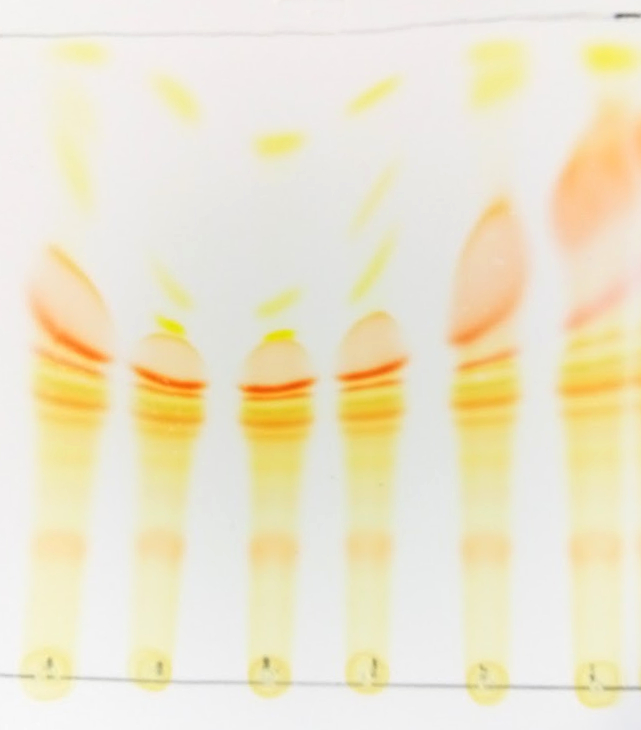
\includegraphics[width=0.5\textwidth]{paprika_editiert.jpg}};
\begin{scope}[x={(image.south east)},y={(image.north west)}]
%% next four lines will help you to locate the point needed by forming a grid. comment these four lines in the final picture.↓
%      \draw[help lines,xstep=.1,ystep=.1] (0,0) grid (1,1);
%        \draw[help lines,xstep=.05,ystep=.05] (0,0) grid (1,1);
%        \foreach \x in {0,1,...,9} { \node [anchor=north] at (\x/10,0) {0.\x}; }
%        \foreach \y in {0,1,...,9} { \node [anchor=east] at (0,\y/10) {0.\y};}
%% upto here↑
\draw[latex-,thick] (0.95,0.98 ) -- +(1cm,0.2cm)node[anchor=west] {\sffamily Fließmittelfront};
\draw[latex-,thick] (0.94,0.75) -- +(2cm,0)node[anchor=west] {\sffamily Substanz};
\draw[latex-,thick] (0.94,0.06) -- +(2cm,0)node[anchor=west] {\sffamily Startpunkt};

\end{scope}
\end{tikzpicture}
	\caption{Dünnschichtchromatographie von Paprikasaft}
	\label{img:paprika}
\end{figure}



\begin{figure}[ht!]
	\centering
	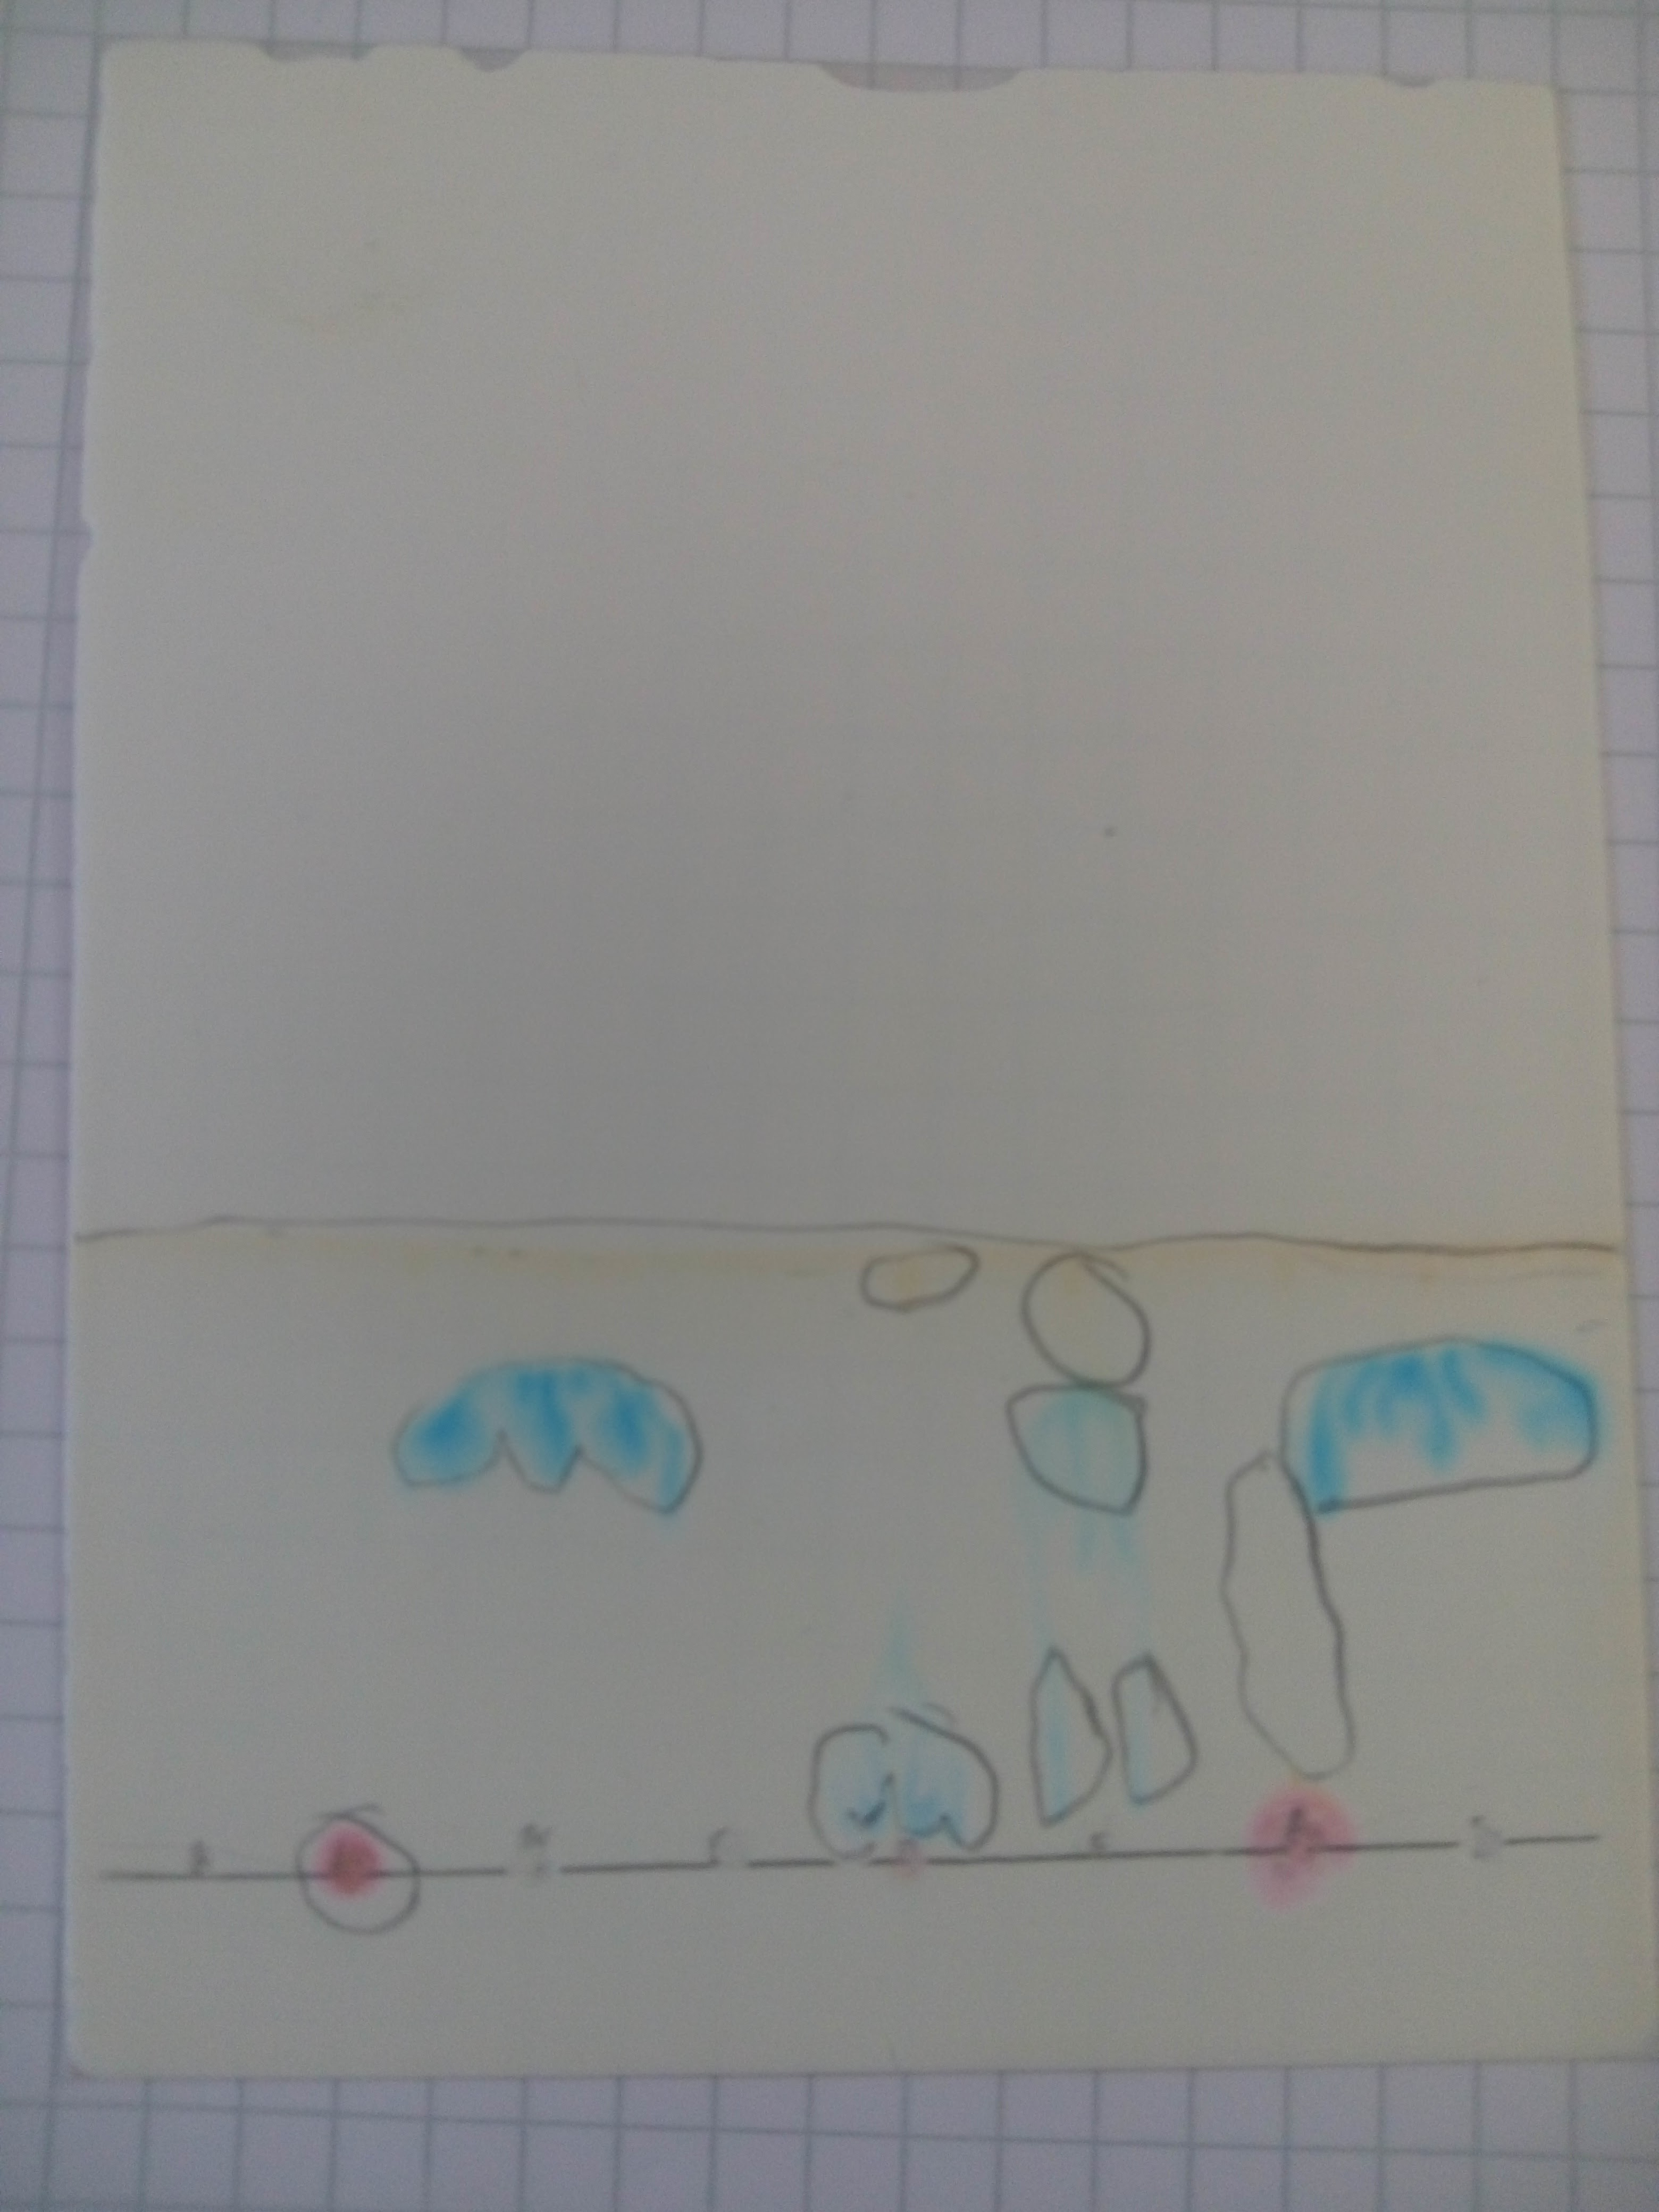
\includegraphics[width=\textwidth]{kieselgel.png}
	\caption{Dünnschichtchromatografie mit Schokolinsen auf einer Kieselgelplatte}
	\label{img: Kieselgel}
\end{figure}

Nach einer Laufzeit von 20 Minuten ist das Laufmittelgemisch, bestehend aus Ethylacetat, Propan-1-ol und Wasser (Verhältniss: 10:60:30) cm an der Kieselgelplatte hochgeflossen.



\begin{figure}[ht!]
\begin{center}
	
	\begin{tikzpicture}
	\begin{axis}[
	draw=none,
	ybar,
	title style={align=center},
	title={Geschmackliche Beurteilung},
	ytick={1, 2.00, 3.00, 4.00, 5.00},
	ylabel=Bewertung,
	xtick=data,
	ymin = 1,
	ymax=5,
axis on top,
height=6cm, width=8cm,
bar width=0.4cm,
ymajorgrids, tick align=inside,
			major grid style={draw=white,line width=1.5pt },
enlarge y limits={value=.1,upper},
enlarge x limits=0.7,
axis x line*=bottom,
axis y line*=left,
y axis line style={opacity=0},
tickwidth=0pt,
legend style={
	at={(0.5,-0.2)},
	anchor=north,
	legend columns=-1,
	/tikz/every even column/.append style={column sep=0.5cm}
},
	symbolic x coords={natürlich,künstlich},
	]
	\addplot[fill=LimeGreen,draw=none] coordinates {(natürlich,3.7) (künstlich, 3.5)};
	\addplot[fill=Goldenrod,draw=none] coordinates {(natürlich,2.9) (künstlich, 3.18)};
	\addplot[fill=BrickRed,draw=none] coordinates {(natürlich,3.7) (künstlich, 3.9)};
	\end{axis}
	\end{tikzpicture}\hfill
	\begin{tikzpicture}
		\begin{axis}[
		draw=none,
		ybar,
		title style={align=center},
		title={Farbigkeit und Aussehen},
		ytick={1, 2.00, 3.00, 4.00, 5.00},
		ylabel=,
		xtick=data,
		ymin = 1,
		ymax=5,
		axis on top,
		height=6cm, width=8cm,
		bar width=0.4cm,
		ymajorgrids, tick align=inside,
			major grid style={draw=white,line width=1.5pt },
		enlarge y limits={value=.1,upper},
		enlarge x limits=0.7,
		axis x line*=bottom,
		axis y line*=left,
		y axis line style={opacity=0},
		tickwidth=0pt,
		legend style={
			at={(0.5,-0.2)},
			anchor=north,
			legend columns=-1,
			/tikz/every even column/.append style={column sep=0.5cm}
		},
		symbolic x coords={natürlich,künstlich},
		]
		\addplot[fill=LimeGreen,draw=none] coordinates {(natürlich,3.63) (künstlich, 3.7)};
		\addplot[fill=Goldenrod,draw=none] coordinates {(natürlich,4.2) (künstlich, 2.9)};
		\addplot[fill=BrickRed,draw=none] coordinates {(natürlich,3.1) (künstlich, 3.7)};
		\end{axis}
		\end{tikzpicture}
		\\[1cm]
		\begin{tikzpicture}
		\pgfplotsset{
			/pgfplots/ybar legend/.style={
				/pgfplots/legend image code/.code={%
					\fill[##1,/tikz/.cd,bar width=3pt,yshift=-0.2em,bar shift=0pt]
					plot coordinates {(0cm,0.8em) (2*\pgfplotbarwidth,0.6em)};},
			}
		}
			\begin{axis}[
			draw=none,
			ybar,
			title style={align=center},
			title={Konsistenz},
			ytick={1, 2.00, 3.00, 4.00, 5.00},
			ylabel=Bewertung,
			xtick=data,
			ymin = 1,
			ymax=5,
			axis on top,
			height=6cm, width=8cm,
			bar width=0.4cm,
			ymajorgrids, tick align=inside,
			major grid style={draw=white,line width=1.5pt },
			enlarge y limits={value=.1,upper},
			enlarge x limits=0.7,
			axis x line*=bottom,
			axis y line*=left,
			y axis line style={opacity=0},
			tickwidth=0pt,
			legend style={
				at={(0.5,-0.2)},
				anchor=north,
				legend columns=-1,
				/tikz/every even column/.append style={column sep=0.5cm}
			},
			symbolic x coords={natürlich,künstlich},
			]
			\addplot[fill=LimeGreen,draw=none] coordinates {(natürlich,3.63) (künstlich, 3.7)};
			\addplot[fill=Goldenrod,draw=none] coordinates {(natürlich,4.2) (künstlich, 2.9)};
			\addplot[fill=BrickRed,draw=none] coordinates {(natürlich,3.1) (künstlich, 3.7)};
			\legend{Grün, Gelb, Rot}
			\end{axis}
			\end{tikzpicture}
\end{center}
\caption[Auswertung der Versuchsreihe mit Lebensmittelfarben]{Auswertung der Versuchsreihe mit gefärbten Muffins. Verwendet wurden sowohl natürliche als auch künstliche Farbstoffe. Die Daten wurden über einen Fragebogen erhoben.}
\label{img:diagram_colors}
\end{figure}


\begin{figure}[htbp]
	\centering
	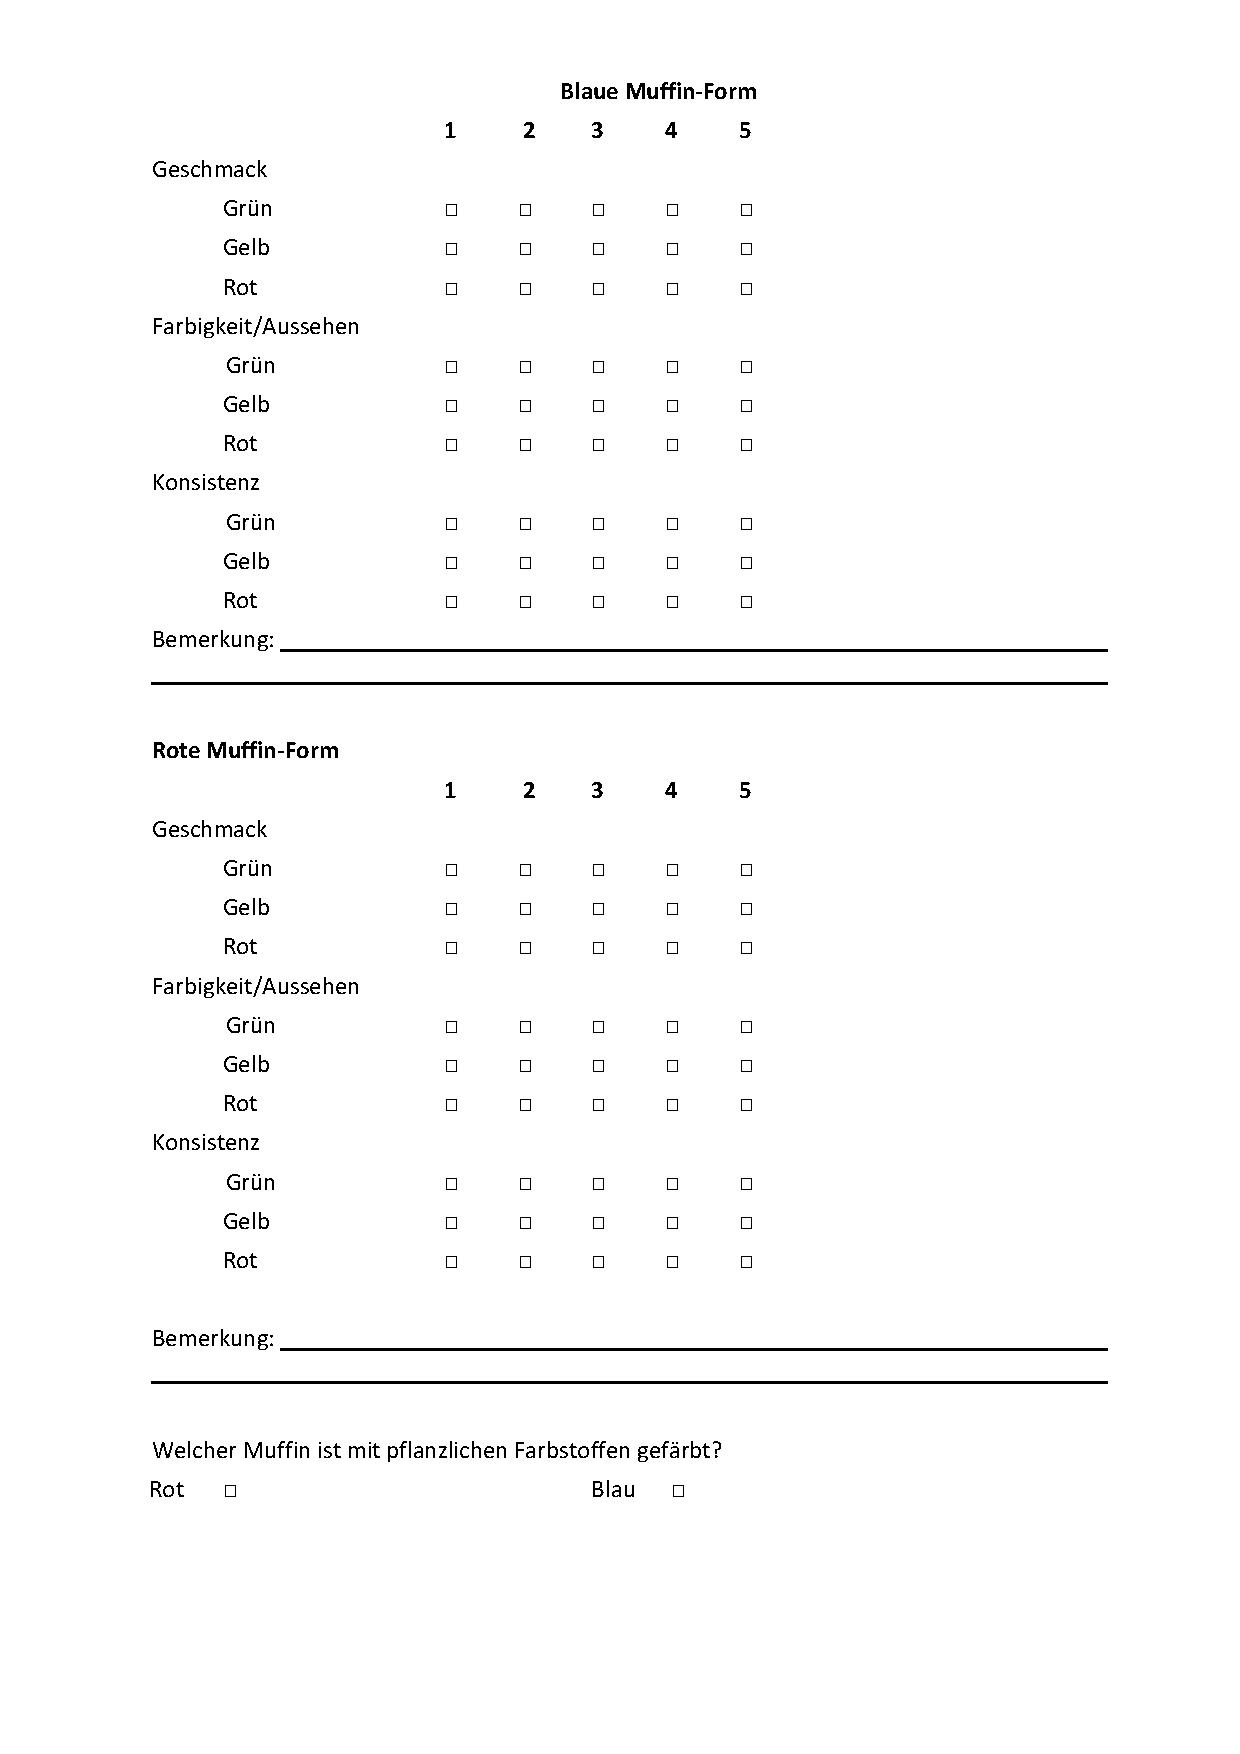
\includegraphics[width=\textwidth]{Fragebogen.pdf}
	\caption{Fragebogen zur Befragung von Probanden, die mit Lebensmittelfarben behandelte Muffins verkostet hatten.}
	\label{img:questions}
\end{figure}


\printbibliography


\chapter*{Eigenständigkeitserklärung}

Ich habe diese Seminararbeit ohne fremde Hilfe angefertigt und nur die im Literaturverzeichnis angeführten Quellen und Hilfsmittel benutzt.

\vspace{2\baselineskip}
\noindent Neuburg, den \today
\par\noindent\makebox[2.5in]{} \hfill\makebox[2.0in]{\hrulefill}%
\par\noindent\makebox[2.5in][l]{} \hfill\makebox[2.0in][l]{Lukas Braun}

\end{document}